\documentclass[]{article}
\usepackage{lmodern}
\usepackage{amssymb,amsmath}
\usepackage{ifxetex,ifluatex}
\usepackage{fixltx2e} % provides \textsubscript
\ifnum 0\ifxetex 1\fi\ifluatex 1\fi=0 % if pdftex
  \usepackage[T1]{fontenc}
  \usepackage[utf8]{inputenc}
\else % if luatex or xelatex
  \ifxetex
    \usepackage{mathspec}
  \else
    \usepackage{fontspec}
  \fi
  \defaultfontfeatures{Ligatures=TeX,Scale=MatchLowercase}
\fi
% use upquote if available, for straight quotes in verbatim environments
\IfFileExists{upquote.sty}{\usepackage{upquote}}{}
% use microtype if available
\IfFileExists{microtype.sty}{%
\usepackage{microtype}
\UseMicrotypeSet[protrusion]{basicmath} % disable protrusion for tt fonts
}{}
\usepackage[margin=1in]{geometry}
\usepackage{hyperref}
\hypersetup{unicode=true,
            pdftitle={Homework 10},
            pdfauthor={Christophe Hunt},
            pdfborder={0 0 0},
            breaklinks=true}
\urlstyle{same}  % don't use monospace font for urls
\usepackage{color}
\usepackage{fancyvrb}
\newcommand{\VerbBar}{|}
\newcommand{\VERB}{\Verb[commandchars=\\\{\}]}
\DefineVerbatimEnvironment{Highlighting}{Verbatim}{commandchars=\\\{\}}
% Add ',fontsize=\small' for more characters per line
\usepackage{framed}
\definecolor{shadecolor}{RGB}{248,248,248}
\newenvironment{Shaded}{\begin{snugshade}}{\end{snugshade}}
\newcommand{\KeywordTok}[1]{\textcolor[rgb]{0.13,0.29,0.53}{\textbf{{#1}}}}
\newcommand{\DataTypeTok}[1]{\textcolor[rgb]{0.13,0.29,0.53}{{#1}}}
\newcommand{\DecValTok}[1]{\textcolor[rgb]{0.00,0.00,0.81}{{#1}}}
\newcommand{\BaseNTok}[1]{\textcolor[rgb]{0.00,0.00,0.81}{{#1}}}
\newcommand{\FloatTok}[1]{\textcolor[rgb]{0.00,0.00,0.81}{{#1}}}
\newcommand{\ConstantTok}[1]{\textcolor[rgb]{0.00,0.00,0.00}{{#1}}}
\newcommand{\CharTok}[1]{\textcolor[rgb]{0.31,0.60,0.02}{{#1}}}
\newcommand{\SpecialCharTok}[1]{\textcolor[rgb]{0.00,0.00,0.00}{{#1}}}
\newcommand{\StringTok}[1]{\textcolor[rgb]{0.31,0.60,0.02}{{#1}}}
\newcommand{\VerbatimStringTok}[1]{\textcolor[rgb]{0.31,0.60,0.02}{{#1}}}
\newcommand{\SpecialStringTok}[1]{\textcolor[rgb]{0.31,0.60,0.02}{{#1}}}
\newcommand{\ImportTok}[1]{{#1}}
\newcommand{\CommentTok}[1]{\textcolor[rgb]{0.56,0.35,0.01}{\textit{{#1}}}}
\newcommand{\DocumentationTok}[1]{\textcolor[rgb]{0.56,0.35,0.01}{\textbf{\textit{{#1}}}}}
\newcommand{\AnnotationTok}[1]{\textcolor[rgb]{0.56,0.35,0.01}{\textbf{\textit{{#1}}}}}
\newcommand{\CommentVarTok}[1]{\textcolor[rgb]{0.56,0.35,0.01}{\textbf{\textit{{#1}}}}}
\newcommand{\OtherTok}[1]{\textcolor[rgb]{0.56,0.35,0.01}{{#1}}}
\newcommand{\FunctionTok}[1]{\textcolor[rgb]{0.00,0.00,0.00}{{#1}}}
\newcommand{\VariableTok}[1]{\textcolor[rgb]{0.00,0.00,0.00}{{#1}}}
\newcommand{\ControlFlowTok}[1]{\textcolor[rgb]{0.13,0.29,0.53}{\textbf{{#1}}}}
\newcommand{\OperatorTok}[1]{\textcolor[rgb]{0.81,0.36,0.00}{\textbf{{#1}}}}
\newcommand{\BuiltInTok}[1]{{#1}}
\newcommand{\ExtensionTok}[1]{{#1}}
\newcommand{\PreprocessorTok}[1]{\textcolor[rgb]{0.56,0.35,0.01}{\textit{{#1}}}}
\newcommand{\AttributeTok}[1]{\textcolor[rgb]{0.77,0.63,0.00}{{#1}}}
\newcommand{\RegionMarkerTok}[1]{{#1}}
\newcommand{\InformationTok}[1]{\textcolor[rgb]{0.56,0.35,0.01}{\textbf{\textit{{#1}}}}}
\newcommand{\WarningTok}[1]{\textcolor[rgb]{0.56,0.35,0.01}{\textbf{\textit{{#1}}}}}
\newcommand{\AlertTok}[1]{\textcolor[rgb]{0.94,0.16,0.16}{{#1}}}
\newcommand{\ErrorTok}[1]{\textcolor[rgb]{0.64,0.00,0.00}{\textbf{{#1}}}}
\newcommand{\NormalTok}[1]{{#1}}
\usepackage{longtable,booktabs}
\usepackage{graphicx,grffile}
\makeatletter
\def\maxwidth{\ifdim\Gin@nat@width>\linewidth\linewidth\else\Gin@nat@width\fi}
\def\maxheight{\ifdim\Gin@nat@height>\textheight\textheight\else\Gin@nat@height\fi}
\makeatother
% Scale images if necessary, so that they will not overflow the page
% margins by default, and it is still possible to overwrite the defaults
% using explicit options in \includegraphics[width, height, ...]{}
\setkeys{Gin}{width=\maxwidth,height=\maxheight,keepaspectratio}
\IfFileExists{parskip.sty}{%
\usepackage{parskip}
}{% else
\setlength{\parindent}{0pt}
\setlength{\parskip}{6pt plus 2pt minus 1pt}
}
\setlength{\emergencystretch}{3em}  % prevent overfull lines
\providecommand{\tightlist}{%
  \setlength{\itemsep}{0pt}\setlength{\parskip}{0pt}}
\setcounter{secnumdepth}{5}
% Redefines (sub)paragraphs to behave more like sections
\ifx\paragraph\undefined\else
\let\oldparagraph\paragraph
\renewcommand{\paragraph}[1]{\oldparagraph{#1}\mbox{}}
\fi
\ifx\subparagraph\undefined\else
\let\oldsubparagraph\subparagraph
\renewcommand{\subparagraph}[1]{\oldsubparagraph{#1}\mbox{}}
\fi

%%% Use protect on footnotes to avoid problems with footnotes in titles
\let\rmarkdownfootnote\footnote%
\def\footnote{\protect\rmarkdownfootnote}

%%% Change title format to be more compact
\usepackage{titling}

% Create subtitle command for use in maketitle
\newcommand{\subtitle}[1]{
  \posttitle{
    \begin{center}\large#1\end{center}
    }
}

\setlength{\droptitle}{-2em}
  \title{Homework 10}
  \pretitle{\vspace{\droptitle}\centering\huge}
  \posttitle{\par}
  \author{Christophe Hunt}
  \preauthor{\centering\large\emph}
  \postauthor{\par}
  \predate{\centering\large\emph}
  \postdate{\par}
  \date{April 3, 2017}

\usepackage{relsize}
\usepackage{setspace}
\usepackage{amsmath,amsfonts,amsthm}
\usepackage[sfdefault]{roboto}
\usepackage[T1]{fontenc}
\usepackage{float}
\usepackage{multirow}
\usepackage{mathtools}
\usepackage{tikz}

\begin{document}
\maketitle

{
\setcounter{tocdepth}{2}
\tableofcontents
}
\section{1. Problem Set}\label{problem-set}

Playing with PageRank You'll verify for yourself that PageRank works by
performing calculations on a small universe of web pages. Let's use the
6 page universe that we had in the course notes.

\begin{figure}[htbp]
\centering
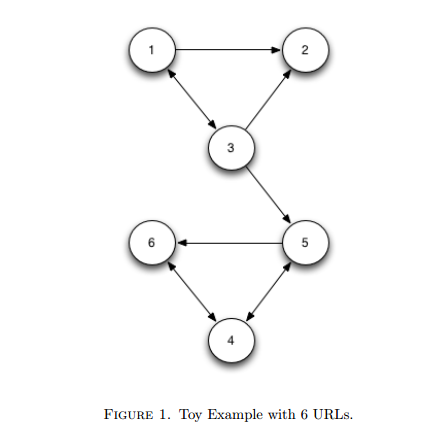
\includegraphics{https://raw.githubusercontent.com/ChristopheHunt/MSDA---Coursework/master/Data\%20605/Assignment\%2010/PS1.PNG}
\caption{}
\end{figure}

For this directed graph, perform the following calculations in \(R\).

\subsection{1}\label{section}

Form the A matrix. Then, introduce decay and form the \(B\) matrix as we
did in the course notes.

\begin{figure}[htbp]
\centering
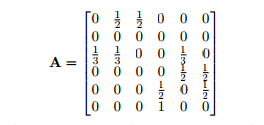
\includegraphics{https://raw.githubusercontent.com/ChristopheHunt/MSDA---Coursework/master/Data\%20605/Assignment\%2010/matrix.PNG}
\caption{}
\end{figure}

\begin{Shaded}
\begin{Highlighting}[]
\NormalTok{A <-}\StringTok{ }\KeywordTok{matrix}\NormalTok{(}\DataTypeTok{data =} \KeywordTok{c}\NormalTok{(}\DecValTok{0}\NormalTok{,}\FloatTok{0.5}\NormalTok{,}\FloatTok{0.5}\NormalTok{,}\DecValTok{0}\NormalTok{,}\DecValTok{0}\NormalTok{,}\DecValTok{0}\NormalTok{, }
                     \DecValTok{0}\NormalTok{,}\DecValTok{0}\NormalTok{,}\DecValTok{0}\NormalTok{,}\DecValTok{0}\NormalTok{,}\DecValTok{0}\NormalTok{,}\DecValTok{0}\NormalTok{,}
                     \FloatTok{0.33}\NormalTok{,}\FloatTok{0.33}\NormalTok{,}\DecValTok{0}\NormalTok{,}\DecValTok{0}\NormalTok{,}\FloatTok{0.33}\NormalTok{,}\DecValTok{0}\NormalTok{,}
                     \DecValTok{0}\NormalTok{,}\DecValTok{0}\NormalTok{,}\DecValTok{0}\NormalTok{,}\DecValTok{0}\NormalTok{,}\FloatTok{0.5}\NormalTok{,}\FloatTok{0.5}\NormalTok{,}
                     \DecValTok{0}\NormalTok{,}\DecValTok{0}\NormalTok{,}\DecValTok{0}\NormalTok{,}\FloatTok{0.5}\NormalTok{,}\DecValTok{0}\NormalTok{,}\FloatTok{0.5}\NormalTok{,}
                     \DecValTok{0}\NormalTok{,}\DecValTok{0}\NormalTok{,}\DecValTok{0}\NormalTok{,}\DecValTok{1}\NormalTok{,}\DecValTok{0}\NormalTok{,}\DecValTok{0}\NormalTok{), }\DataTypeTok{nrow =} \DecValTok{6}\NormalTok{,  }\DataTypeTok{byrow =} \OtherTok{TRUE}\NormalTok{)}
\NormalTok{A}
\end{Highlighting}
\end{Shaded}

\begin{longtable}[]{@{}rrrrrr@{}}
\toprule
0.00 & 0.50 & 0.5 & 0.0 & 0.00 & 0.0\tabularnewline
0.00 & 0.00 & 0.0 & 0.0 & 0.00 & 0.0\tabularnewline
0.33 & 0.33 & 0.0 & 0.0 & 0.33 & 0.0\tabularnewline
0.00 & 0.00 & 0.0 & 0.0 & 0.50 & 0.5\tabularnewline
0.00 & 0.00 & 0.0 & 0.5 & 0.00 & 0.5\tabularnewline
0.00 & 0.00 & 0.0 & 1.0 & 0.00 & 0.0\tabularnewline
\bottomrule
\end{longtable}

\begin{quote}
Now we introduce decay to create the \(B\) matrix using the equation:
\(B = 0.85 * A + \frac{0.15}{n}\)
\end{quote}

\begin{Shaded}
\begin{Highlighting}[]
\NormalTok{B <-}\StringTok{ }\FloatTok{0.85} \NormalTok{*}\StringTok{ }\NormalTok{A +}\StringTok{ }\NormalTok{.}\DecValTok{15} \NormalTok{/}\StringTok{ }\KeywordTok{nrow}\NormalTok{(A)}
\NormalTok{B}
\end{Highlighting}
\end{Shaded}

\begin{longtable}[]{@{}rrrrrr@{}}
\toprule
0.0250 & 0.4500 & 0.450 & 0.025 & 0.0250 & 0.025\tabularnewline
0.0250 & 0.0250 & 0.025 & 0.025 & 0.0250 & 0.025\tabularnewline
0.3055 & 0.3055 & 0.025 & 0.025 & 0.3055 & 0.025\tabularnewline
0.0250 & 0.0250 & 0.025 & 0.025 & 0.4500 & 0.450\tabularnewline
0.0250 & 0.0250 & 0.025 & 0.450 & 0.0250 & 0.450\tabularnewline
0.0250 & 0.0250 & 0.025 & 0.875 & 0.0250 & 0.025\tabularnewline
\bottomrule
\end{longtable}

\subsection{2}\label{section-1}

Start with a uniform rank vector r and perform power iterations on B
till convergence. That is, compute the solution \(r = B^n * r\). Attempt
this for a sufficiently large \(n\) so that \(r\) actually converges.

\begin{quote}
Following our notes, we assume equal probability of a user clicking a
link so we start with the rank vector r is
\(r = (.167, .167, .167, .167, .167, .167)\)
\end{quote}

\begin{Shaded}
\begin{Highlighting}[]
\KeywordTok{library}\NormalTok{(expm) }
\end{Highlighting}
\end{Shaded}

\begin{verbatim}
## Warning: package 'expm' was built under R version 3.3.3
\end{verbatim}

\begin{verbatim}
## Loading required package: Matrix
\end{verbatim}

\begin{verbatim}
## 
## Attaching package: 'expm'
\end{verbatim}

\begin{verbatim}
## The following object is masked from 'package:Matrix':
## 
##     expm
\end{verbatim}

\begin{Shaded}
\begin{Highlighting}[]
\NormalTok{r <-}\StringTok{ }\KeywordTok{c}\NormalTok{(.}\DecValTok{167}\NormalTok{, .}\DecValTok{167}\NormalTok{, .}\DecValTok{167}\NormalTok{, .}\DecValTok{167}\NormalTok{, .}\DecValTok{167}\NormalTok{, .}\DecValTok{167}\NormalTok{)}
\NormalTok{n <-}\StringTok{ }\DecValTok{40}
\NormalTok{(B %^%}\StringTok{ }\NormalTok{n) %*%}\StringTok{ }\NormalTok{r}
\end{Highlighting}
\end{Shaded}

\begin{longtable}[]{@{}r@{}}
\toprule
0.0100757\tabularnewline
0.0026836\tabularnewline
0.0138653\tabularnewline
0.0251686\tabularnewline
0.0251686\tabularnewline
0.0251686\tabularnewline
\bottomrule
\end{longtable}

\begin{Shaded}
\begin{Highlighting}[]
\NormalTok{A %*%}\StringTok{ }\NormalTok{r}
\end{Highlighting}
\end{Shaded}

\begin{longtable}[]{@{}r@{}}
\toprule
0.16700\tabularnewline
0.00000\tabularnewline
0.16533\tabularnewline
0.16700\tabularnewline
0.16700\tabularnewline
0.16700\tabularnewline
\bottomrule
\end{longtable}

\subsection{3}\label{section-2}

Compute the eigen-decomposition of \(B\) and verify that you indeed get
an eigenvalue of 1 as the largest eigenvalue and that its corresponding
eigenvector is the same vector that you obtained in the previous power
iteration method. Further, this eigenvector has all positive entries and
it sums to 1.

\newpage

\subsection{4}\label{section-3}

\begin{Shaded}
\begin{Highlighting}[]
\KeywordTok{library}\NormalTok{(igraph)}
\end{Highlighting}
\end{Shaded}

Use the \(graph\) package in R and its \(page.rank\) method to compute
the Page Rank of the graph as given in A. Note that you don't need to
apply decay. The package starts with a connected graph and applies decay
internally. Verify that you do get the same PageRank vector as the two
approaches above. Please document all your experiments in an R Markdown
document.

\begin{Shaded}
\begin{Highlighting}[]
\KeywordTok{library}\NormalTok{(igraph)}
\NormalTok{df <-}\StringTok{ }\KeywordTok{data.frame}\NormalTok{(}\DataTypeTok{from=}\KeywordTok{c}\NormalTok{(}\DecValTok{1}\NormalTok{,}\DecValTok{1}\NormalTok{,}\DecValTok{3}\NormalTok{,}\DecValTok{3}\NormalTok{,}\DecValTok{3}\NormalTok{,}\DecValTok{4}\NormalTok{,}\DecValTok{4}\NormalTok{,}\DecValTok{5}\NormalTok{,}\DecValTok{5}\NormalTok{,}\DecValTok{6}\NormalTok{),}
                 \DataTypeTok{to =} \KeywordTok{c}\NormalTok{(}\DecValTok{2}\NormalTok{,}\DecValTok{3}\NormalTok{,}\DecValTok{1}\NormalTok{,}\DecValTok{2}\NormalTok{,}\DecValTok{5}\NormalTok{,}\DecValTok{5}\NormalTok{,}\DecValTok{6}\NormalTok{,}\DecValTok{4}\NormalTok{,}\DecValTok{6}\NormalTok{,}\DecValTok{4}\NormalTok{),}
             \DataTypeTok{weight =} \KeywordTok{c}\NormalTok{(}\DecValTok{1}\NormalTok{,}\DecValTok{1}\NormalTok{,}\DecValTok{1}\NormalTok{,}\DecValTok{1}\NormalTok{,}\DecValTok{1}\NormalTok{,}\DecValTok{1}\NormalTok{,}\DecValTok{1}\NormalTok{,}\DecValTok{1}\NormalTok{,}\DecValTok{1}\NormalTok{,}\DecValTok{1}\NormalTok{))}
\NormalTok{g <-}\StringTok{ }\KeywordTok{graph.data.frame}\NormalTok{(df, }\DataTypeTok{directed =} \OtherTok{TRUE}\NormalTok{)}
\NormalTok{results <-}\StringTok{ }\KeywordTok{page_rank}\NormalTok{(g, }\DataTypeTok{algo =} \KeywordTok{c}\NormalTok{(}\StringTok{"power"}\NormalTok{))}
\NormalTok{v <-}\StringTok{ }\KeywordTok{matrix}\NormalTok{(results$vector, }\DataTypeTok{ncol =} \DecValTok{1}\NormalTok{)}
\NormalTok{v}
\end{Highlighting}
\end{Shaded}

\begin{longtable}[]{@{}r@{}}
\toprule
0.0395097\tabularnewline
0.0440479\tabularnewline
0.3705699\tabularnewline
0.2052394\tabularnewline
0.2833665\tabularnewline
0.0572665\tabularnewline
\bottomrule
\end{longtable}

\begin{Shaded}
\begin{Highlighting}[]
\NormalTok{igraph::}\KeywordTok{plot.igraph}\NormalTok{(g)}
\end{Highlighting}
\end{Shaded}

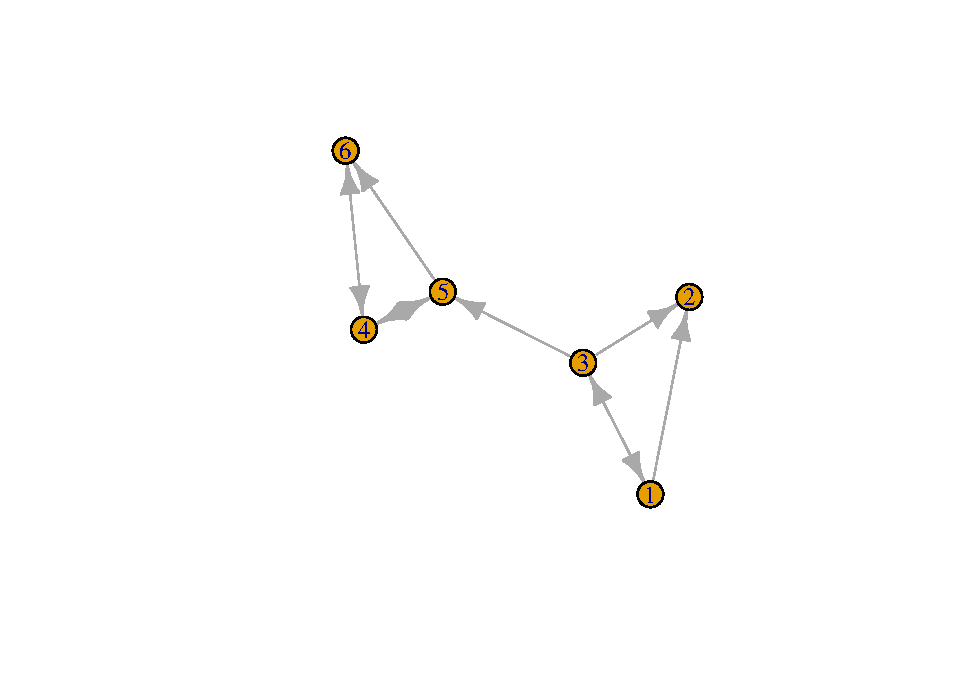
\includegraphics{CHunt_Assign10_PS1_files/figure-latex/unnamed-chunk-8-1.pdf}


\end{document}
